%-*-latex-*-
\tinysidebar{\debug{exercises/20-n5-n3-1-5n3-cos-n-7-8/answer.tex}}
(a)
Let $f_0(n) = 20 n^5/(n^3 + 1)$.
The following is a plot of $|f_0(n)|$ and $20n^2$:
%-*-latex-*-

\begin{center}
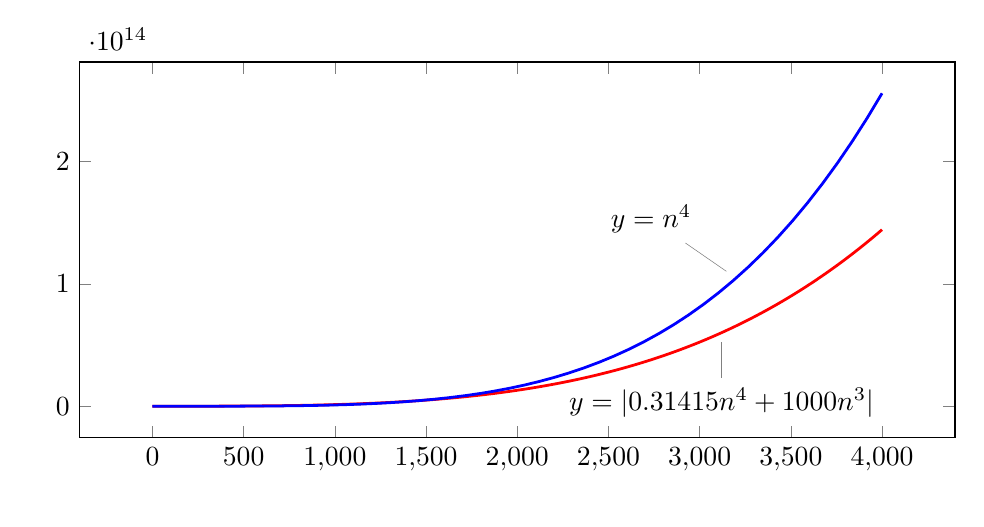
\begin{tikzpicture}[line width=1]
\begin{axis}[width=5in, height=2.5in,
             scatter/classes={a={mark=*,draw=black}},
             xlabel={\mbox{}},
             xlabel style={name=xlabel}, 
             ylabel={\mbox{}}, 
             legend style={
                at={(xlabel.south)},
                yshift=-1ex,
                anchor=north,
                legend cell align=left,
                },
        ]
]
\addplot[draw=red, line width=1] coordinates {(0.0,0.0)
(4.004,64273.1295)
(8.008,514830.9955)
(12.012,1739734.7218)
(16.016,4128983.3103)
(20.02,8074513.6398)
(24.024,13970200.4669)
(28.028,22211856.4258)
(32.032,33197232.0279)
(36.036,47326015.6622)
(40.04,64999833.5953)
(44.044,86622249.9712)
(48.048,112598766.8113)
(52.0521,143336824.0147)
(56.0561,179245799.3578)
(60.0601,220737008.4947)
(64.0641,268223704.9566)
(68.0681,322121080.1527)
(72.0721,382846263.3693)
(76.0761,450818321.7704)
(80.0801,526458260.3973)
(84.0841,610189022.1691)
(88.0881,702435487.882)
(92.0921,803624476.2101)
(96.0961,914184743.7046)
(100.1001,1034546984.7944)
(104.1041,1165143831.786)
(108.1081,1306409854.8631)
(112.1121,1458781562.087)
(116.1161,1622697399.3968)
(120.1201,1798597750.6085)
(124.1241,1986924937.4162)
(128.1281,2188123219.391)
(132.1321,2402638793.9817)
(136.1361,2630919796.5147)
(140.1401,2873416300.1938)
(144.1441,3130580316.1001)
(148.1481,3402865793.1925)
(152.1522,3690728618.3071)
(156.1562,3994626616.1578)
(160.1602,4315019549.3358)
(164.1642,4652369118.3098)
(168.1682,5007138961.4259)
(172.1722,5379794654.9079)
(176.1762,5770803712.857)
(180.1802,6180635587.2518)
(184.1842,6609761667.9486)
(188.1882,7058655282.681)
(192.1922,7527791697.0601)
(196.1962,8017648114.5746)
(200.2002,8528703676.5906)
(204.2042,9061439462.3517)
(208.2082,9616338488.9791)
(212.2122,10193885711.4714)
(216.2162,10794568022.7046)
(220.2202,11418874253.4323)
(224.2242,12067295172.2856)
(228.2282,12740323485.7731)
(232.2322,13438453838.2809)
(236.2362,14162182812.0724)
(240.2402,14912008927.2887)
(244.2442,15688432641.9484)
(248.2482,16491956351.9474)
(252.2523,17323084391.0593)
(256.2563,18182323030.9351)
(260.2603,19070180481.1032)
(264.2643,19987166888.9696)
(268.2683,20933794339.8179)
(272.2723,21910576856.8089)
(276.2763,22918030400.9811)
(280.2803,23956672871.2505)
(284.2843,25027024104.4105)
(288.2883,26129605875.132)
(292.2923,27264941895.9634)
(296.2963,28433557817.3306)
(300.3003,29635981227.5371)
(304.3043,30872741652.7636)
(308.3083,32144370557.0687)
(312.3123,33451401342.388)
(316.3163,34794369348.5351)
(320.3203,36173811853.2007)
(324.3243,37590268071.9532)
(328.3283,39044279158.2384)
(332.3323,40536388203.3797)
(336.3363,42067140236.5778)
(340.3403,43637082224.911)
(344.3443,45246763073.3351)
(348.3483,46896733624.6834)
(352.3524,48587546659.6667)
(356.3564,50319756896.8732)
(360.3604,52093920992.7687)
(364.3644,53910597541.6964)
(368.3684,55770347075.877)
(372.3724,57673732065.4089)
(376.3764,59621316918.2676)
(380.3804,61613667980.3064)
(384.3844,63651353535.2559)
(388.3884,65734943804.7245)
(392.3924,67865010948.1976)
(396.3964,70042129063.0386)
(400.4004,72266874184.488)
(404.4044,74539824285.6641)
(408.4084,76861559277.5623)
(412.4124,79232661009.0559)
(416.4164,81653713266.8955)
(420.4204,84125301775.7092)
(424.4244,86648014198.0026)
(428.4284,89222440134.1587)
(432.4324,91849171122.4382)
(436.4364,94528800638.9791)
(440.4404,97261924097.797)
(444.4444,100049138850.7849)
(448.4484,102891044187.7133)
(452.4525,105788241336.2304)
(456.4565,108741333461.8616)
(460.4605,111750925668.0099)
(464.4645,114817624995.9558)
(468.4685,117942040424.8574)
(472.4725,121124782871.7501)
(476.4765,124366465191.5468)
(480.4805,127667702177.0381)
(484.4845,131029110558.8919)
(488.4885,134451309005.6537)
(492.4925,137934918123.7463)
(496.4965,141480560457.4702)
(500.5005,145088860489.0033)
(504.5045,148760444638.4011)
(508.5085,152495941263.5963)
(512.5125,156295980660.3996)
(516.5165,160161195062.4986)
(520.5205,164092218641.4588)
(524.5245,168089687506.723)
(528.5285,172154239705.6116)
(532.5325,176286515223.3223)
(536.5365,180487155982.9306)
(540.5405,184756805845.3893)
(544.5445,189096110609.5286)
(548.5485,193505718012.0564)
(552.5526,197986277727.558)
(556.5566,202538441368.496)
(560.5606,207162862485.2109)
(564.5646,211860196565.9203)
(568.5686,216631101036.7197)
(572.5726,221476235261.5815)
(576.5766,226396260542.3562)
(580.5806,231391840118.7714)
(584.5846,236463639168.4324)
(588.5886,241612324806.8218)
(592.5926,246838566087.2999)
(596.5966,252143034001.1042)
(600.6006,257526401477.3502)
(604.6046,262989343383.0303)
(608.6086,268532536523.0147)
(612.6126,274156659640.0511)
(616.6166,279862393414.7646)
(620.6206,285650420465.658)
(624.6246,291521425349.1111)
(628.6286,297476094559.3817)
(632.6326,303515116528.605)
(636.6366,309639181626.7935)
(640.6406,315848982161.8371)
(644.6446,322145212379.5036)
(648.6486,328528568463.438)
(652.6527,334999748535.1628)
(656.6567,341559452654.0781)
(660.6607,348208382817.4615)
(664.6647,354947242960.468)
(668.6687,361776738956.1299)
(672.6727,368697578615.3575)
(676.6767,375710471686.938)
(680.6807,382816129857.5367)
(684.6847,390015266751.6959)
(688.6887,397308597931.8356)
(692.6927,404696840898.2532)
(696.6967,412180715089.1237)
(700.7007,419760941880.4995)
(704.7047,427438244586.3107)
(708.7087,435213348458.3644)
(712.7127,443086980686.3458)
(716.7167,451059870397.8172)
(720.7207,459132748658.2184)
(724.7247,467306348470.8671)
(728.7287,475581404776.9576)
(732.7327,483958654455.5628)
(736.7367,492438836323.6323)
(740.7407,501022691135.9935)
(744.7447,509710961585.3513)
(748.7487,518504392302.2878)
(752.7528,527403729855.2631)
(756.7568,536409722750.6143)
(760.7608,545523121432.5563)
(764.7648,554744678283.1813)
(768.7688,564075147622.4592)
(772.7728,573515285708.237)
(776.7768,583065850736.2399)
(780.7808,592727602840.0698)
(784.7848,602501304091.2065)
(788.7888,612387718499.0072)
(792.7928,622387612010.7068)
(796.7968,632501752511.4172)
(800.8008,642730909824.1285)
(804.8048,653075855709.7076)
(808.8088,663537363866.8992)
(812.8128,674116209932.3257)
(816.8168,684813171480.4865)
(820.8208,695629028023.7587)
(824.8248,706564561012.3973)
(828.8288,717620553834.534)
(832.8328,728797791816.1787)
(836.8368,740097062221.2186)
(840.8408,751519154251.418)
(844.8448,763064859046.4193)
(848.8488,774734969683.7417)
(852.8529,786530281178.7827)
(856.8569,798451590484.8167)
(860.8609,810499696492.9956)
(864.8649,822675400032.3492)
(868.8689,834979503869.7843)
(872.8729,847412812710.0857)
(876.8769,859976133195.915)
(880.8809,872670273907.8123)
(884.8849,885496045364.194)
(888.8889,898454260021.355)
(892.8929,911545732273.467)
(896.8969,924771278452.5798)
(900.9009,938131716828.62)
(904.9049,951627867609.3923)
(908.9089,965260552940.5784)
(912.9129,979030596905.738)
(916.9169,992938825526.308)
(920.9209,1006986066761.6028)
(924.9249,1021173150508.814)
(928.9289,1035500908603.0114)
(932.9329,1049970174817.1416)
(936.9369,1064581784862.029)
(940.9409,1079336576386.3757)
(944.9449,1094235388976.761)
(948.9489,1109279064157.6414)
(952.953,1124468445391.3516)
(956.957,1139804378078.1035)
(960.961,1155287709555.9858)
(964.965,1170919289100.966)
(968.969,1186699967926.8882)
(972.973,1202630599185.474)
(976.977,1218712037966.323)
(980.981,1234945141296.9116)
(984.985,1251330768142.5942)
(988.989,1267869779406.6025)
(992.993,1284563037930.046)
(996.997,1301411408491.9111)
(1001.001,1318415757809.0625)
(1005.005,1335576954536.2412)
(1009.009,1352895869266.0671)
(1013.013,1370373374529.0364)
(1017.017,1388010344793.5234)
(1021.021,1405807656465.7803)
(1025.025,1423766187889.9348)
(1029.029,1441886819347.9946)
(1033.033,1460170433059.8442)
(1037.037,1478617913183.2446)
(1041.041,1497230145813.835)
(1045.045,1516008018985.1323)
(1049.049,1534952422668.5303)
(1053.0531,1554064248773.301)
(1057.0571,1573344391146.5933)
(1061.0611,1592793745573.4336)
(1065.0651,1612413209776.726)
(1069.0691,1632203683417.2524)
(1073.0731,1652166068093.6714)
(1077.0771,1672301267342.5203)
(1081.0811,1692610186638.212)
(1085.0851,1713093733393.039)
(1089.0891,1733752816957.17)
(1093.0931,1754588348618.651)
(1097.0971,1775601241603.4065)
(1101.1011,1796792411075.2378)
(1105.1051,1818162774135.8245)
(1109.1091,1839713249824.7222)
(1113.1131,1861444759119.3655)
(1117.1171,1883358224935.0654)
(1121.1211,1905454572125.0105)
(1125.1251,1927734727480.268)
(1129.1291,1950199619729.7817)
(1133.1331,1972850179540.3726)
(1137.1371,1995687339516.7402)
(1141.1411,2018712034201.46)
(1145.1451,2041925200074.9866)
(1149.1491,2065327775555.6511)
(1153.1532,2088920700999.6626)
(1157.1572,2112704918701.1072)
(1161.1612,2136681372891.9487)
(1165.1652,2160851009742.0286)
(1169.1692,2185214777359.0654)
(1173.1732,2209773625788.6562)
(1177.1772,2234528507014.274)
(1181.1812,2259480374957.27)
(1185.1852,2284630185476.874)
(1189.1892,2309978896370.1914)
(1193.1932,2335527467372.206)
(1197.1972,2361276860155.7793)
(1201.2012,2387228038331.6494)
(1205.2052,2413381967448.4336)
(1209.2092,2439739614992.6255)
(1213.2132,2466301950388.5957)
(1217.2172,2493069944998.593)
(1221.2212,2520044572122.744)
(1225.2252,2547226806999.052)
(1229.2292,2574617626803.398)
(1233.2332,2602218010649.541)
(1237.2372,2630028939589.1177)
(1241.2412,2658051396611.6406)
(1245.2452,2686286366644.502)
(1249.2492,2714734836552.9697)
(1253.2533,2743397795140.1895)
(1257.2573,2772276233147.1865)
(1261.2613,2801371143252.8604)
(1265.2653,2830683520073.99)
(1269.2693,2860214360165.2324)
(1273.2733,2889964662019.12)
(1277.2773,2919935426066.0645)
(1281.2813,2950127654674.354)
(1285.2853,2980542352150.155)
(1289.2893,3011180524737.5103)
(1293.2933,3042043180618.342)
(1297.2973,3073131329912.4473)
(1301.3013,3104445984677.504)
(1305.3053,3135988158909.0645)
(1309.3093,3167758868540.5596)
(1313.3133,3199759131443.2974)
(1317.3173,3231989967426.465)
(1321.3213,3264452398237.125)
(1325.3253,3297147447560.219)
(1329.3293,3330076141018.5654)
(1333.3333,3363239506172.8594)
(1337.3373,3396638572521.675)
(1341.3413,3430274371501.464)
(1345.3453,3464147936486.5527)
(1349.3493,3498260302789.1475)
(1353.3534,3532612507659.333)
(1357.3574,3567205590285.0703)
(1361.3614,3602040591792.196)
(1365.3654,3637118555244.427)
(1369.3694,3672440525643.3564)
(1373.3734,3708007549928.455)
(1377.3774,3743820676977.0713)
(1381.3814,3779880957604.4316)
(1385.3854,3816189444563.638)
(1389.3894,3852747192545.672)
(1393.3934,3889555258179.392)
(1397.3974,3926614700031.534)
(1401.4014,3963926578606.711)
(1405.4054,4001491956347.413)
(1409.4094,4039311897634.0093)
(1413.4134,4077387468784.745)
(1417.4174,4115719738055.744)
(1421.4214,4154309775641.006)
(1425.4254,4193158653672.4097)
(1429.4294,4232267446219.711)
(1433.4334,4271637229290.543)
(1437.4374,4311269080830.417)
(1441.4414,4351164080722.7197)
(1445.4454,4391323310788.718)
(1449.4494,4431747854787.555)
(1453.4535,4472438798416.25)
(1457.4575,4513397229309.703)
(1461.4615,4554624237040.688)
(1465.4655,4596120913119.859)
(1469.4695,4637888350995.748)
(1473.4735,4679927646054.76)
(1477.4775,4722239895621.183)
(1481.4815,4764826198957.178)
(1485.4855,4807687657262.787)
(1489.4895,4850825373675.929)
(1493.4935,4894240453272.396)
(1497.4975,4937934003065.865)
(1501.5015,4981907132007.886)
(1505.5055,5026160950987.885)
(1509.5095,5070696572833.168)
(1513.5135,5115515112308.919)
(1517.5175,5160617686118.197)
(1521.5215,5206005412901.942)
(1525.5255,5251679413238.969)
(1529.5295,5297640809645.969)
(1533.5335,5343890726577.515)
(1537.5375,5390430290426.053)
(1541.5415,5437260629521.909)
(1545.5455,5484382874133.286)
(1549.5495,5531798156466.265)
(1553.5536,5579507610664.803)
(1557.5576,5627512372810.736)
(1561.5616,5675813580923.777)
(1565.5656,5724412374961.517)
(1569.5696,5773309896819.421)
(1573.5736,5822507290330.838)
(1577.5776,5872005701266.987)
(1581.5816,5921806277336.973)
(1585.5856,5971910168187.77)
(1589.5896,6022318525404.234)
(1593.5936,6073032502509.099)
(1597.5976,6124053254962.976)
(1601.6016,6175381940164.35)
(1605.6056,6227019717449.588)
(1609.6096,6278967748092.933)
(1613.6136,6331227195306.505)
(1617.6176,6383799224240.301)
(1621.6216,6436685001982.197)
(1625.6256,6489885697557.945)
(1629.6296,6543402481931.178)
(1633.6336,6597236528003.398)
(1637.6376,6651389010613.996)
(1641.6416,6705861106540.232)
(1645.6456,6760653994497.246)
(1649.6496,6815768855138.057)
(1653.6537,6871206871053.56)
(1657.6577,6926969226772.525)
(1661.6617,6983057108761.606)
(1665.6657,7039471705425.328)
(1669.6697,7096214207106.098)
(1673.6737,7153285806084.197)
(1677.6777,7210687696577.785)
(1681.6817,7268421074742.9)
(1685.6857,7326487138673.459)
(1689.6897,7384887088401.252)
(1693.6937,7443622125895.949)
(1697.6977,7502693455065.102)
(1701.7017,7562102281754.129)
(1705.7057,7621849813746.338)
(1709.7097,7681937260762.906)
(1713.7137,7742365834462.893)
(1717.7177,7803136748443.232)
(1721.7217,7864251218238.736)
(1725.7257,7925710461322.096)
(1729.7297,7987515697103.879)
(1733.7337,8049668146932.529)
(1737.7377,8112169034094.369)
(1741.7417,8175019583813.6)
(1745.7457,8238221023252.297)
(1749.7497,8301774581510.417)
(1753.7538,8365681489625.793)
(1757.7578,8429942980574.135)
(1761.7618,8494560289269.026)
(1765.7658,8559534652561.936)
(1769.7698,8624867309242.203)
(1773.7738,8690559500037.053)
(1777.7778,8756612467611.578)
(1781.7818,8823027456568.754)
(1785.7858,8889805713449.436)
(1789.7898,8956948486732.35)
(1793.7938,9024457026834.105)
(1797.7978,9092332586109.188)
(1801.8018,9160576418849.957)
(1805.8058,9229189781286.654)
(1809.8098,9298173931587.398)
(1813.8138,9367530129858.182)
(1817.8178,9437259638142.877)
(1821.8218,9507363720423.234)
(1825.8258,9577843642618.885)
(1829.8298,9648700672587.326)
(1833.8338,9719936080123.943)
(1837.8378,9791551136961.998)
(1841.8418,9863547116772.625)
(1845.8458,9935925295164.84)
(1849.8498,10008686949685.535)
(1853.8539,10081833359819.484)
(1857.8579,10155365806989.326)
(1861.8619,10229285574555.59)
(1865.8659,10303593947816.68)
(1869.8699,10378292214008.871)
(1873.8739,10453381662306.326)
(1877.8779,10528863583821.074)
(1881.8819,10604739271603.03)
(1885.8859,10681010020639.982)
(1889.8899,10757677127857.6)
(1893.8939,10834741892119.426)
(1897.8979,10912205614226.883)
(1901.9019,10990069596919.27)
(1905.9059,11068335144873.766)
(1909.9099,11147003564705.422)
(1913.9139,11226076164967.172)
(1917.9179,11305554256149.828)
(1921.9219,11385439150682.072)
(1925.9259,11465732162930.473)
(1929.9299,11546434609199.47)
(1933.9339,11627547807731.385)
(1937.9379,11709073078706.414)
(1941.9419,11791011744242.629)
(1945.9459,11873365128395.984)
(1949.9499,11956134557160.312)
(1953.954,12039321358467.312)
(1957.958,12122926862186.578)
(1961.962,12206952400125.562)
(1965.966,12291399306029.61)
(1969.97,12376268915581.938)
(1973.974,12461562566403.64)
(1977.978,12547281598053.688)
(1981.982,12633427352028.93)
(1985.986,12720001171764.094)
(1989.99,12807004402631.781)
(1993.994,12894438391942.479)
(1997.998,12982304488944.543)
(2002.002,13070604044824.21)
(2006.006,13159338412705.6)
(2010.01,13248508947650.697)
(2014.014,13338117006659.375)
(2018.018,13428163948669.379)
(2022.022,13518651134556.332)
(2026.026,13609579927133.738)
(2030.03,13700951691152.977)
(2034.034,13792767793303.305)
(2038.038,13885029602211.854)
(2042.042,13977738488443.637)
(2046.046,14070895824501.545)
(2050.0501,14164502984826.344)
(2054.0541,14258561345796.676)
(2058.0581,14353072285729.066)
(2062.0621,14448037184877.908)
(2066.0661,14543457425435.484)
(2070.0701,14639334391531.95)
(2074.0741,14735669469235.328)
(2078.0781,14832464046551.54)
(2082.0821,14929719513424.36)
(2086.0861,15027437261735.459)
(2090.0901,15125618685304.379)
(2094.0941,15224265179888.54)
(2098.0981,15323378143183.229)
(2102.1021,15422958974821.633)
(2106.1061,15523009076374.797)
(2110.1101,15623529851351.652)
(2114.1141,15724522705198.998)
(2118.1181,15825989045301.531)
(2122.1221,15927930280981.803)
(2126.1261,16030347823500.26)
(2130.1301,16133243086055.21)
(2134.1341,16236617483782.854)
(2138.1381,16340472433757.262)
(2142.1421,16444809354990.383)
(2146.1461,16549629668432.04)
(2150.1502,16654934796969.94)
(2154.1542,16760726165429.664)
(2158.1582,16867005200574.672)
(2162.1622,16973773331106.303)
(2166.1662,17081031987663.762)
(2170.1702,17188782602824.148)
(2174.1742,17297026611102.43)
(2178.1782,17405765448951.45)
(2182.1822,17515000554761.934)
(2186.1862,17624733368862.484)
(2190.1902,17734965333519.582)
(2194.1942,17845697892937.58)
(2198.1982,17956932493258.707)
(2202.2022,18068670582563.086)
(2206.2062,18180913610868.695)
(2210.2102,18293663030131.41)
(2214.2142,18406920294244.97)
(2218.2182,18520686859040.992)
(2222.2222,18634964182288.984)
(2226.2262,18749753723696.312)
(2230.2302,18865056944908.242)
(2234.2342,18980875309507.9)
(2238.2382,19097210283016.285)
(2242.2422,19214063332892.297)
(2246.2462,19331435928532.69)
(2250.2503,19449329541272.117)
(2254.2543,19567745644383.082)
(2258.2583,19686685713075.992)
(2262.2623,19806151224499.117)
(2266.2663,19926143657738.61)
(2270.2703,20046664493818.496)
(2274.2743,20167715215700.684)
(2278.2783,20289297308284.957)
(2282.2823,20411412258408.977)
(2286.2863,20534061554848.28)
(2290.2903,20657246688316.285)
(2294.2943,20780969151464.285)
(2298.2983,20905230438881.453)
(2302.3023,21030032047094.832)
(2306.3063,21155375474569.35)
(2310.3103,21281262221707.812)
(2314.3143,21407693790850.906)
(2318.3183,21534671686277.18)
(2322.3223,21662197414203.074)
(2326.3263,21790272482782.9)
(2330.3303,21918898402108.85)
(2334.3343,22048076684210.996)
(2338.3383,22177808843057.28)
(2342.3423,22308096394553.523)
(2346.3463,22438940856543.438)
(2350.3504,22570343748808.586)
(2354.3544,22702306593068.438)
(2358.3584,22834830912980.32)
(2362.3624,22967918234139.44)
(2366.3664,23101570084078.9)
(2370.3704,23235787992269.65)
(2374.3744,23370573490120.54)
(2378.3784,23505928110978.293)
(2382.3824,23641853390127.508)
(2386.3864,23778350864790.656)
(2390.3904,23915422074128.094)
(2394.3944,24053068559238.05)
(2398.3984,24191291863156.637)
(2402.4024,24330093530857.836)
(2406.4064,24469475109253.516)
(2410.4104,24609438147193.406)
(2414.4144,24749984195465.14)
(2418.4184,24891114806794.207)
(2422.4224,25032831535843.977)
(2426.4264,25175135939215.707)
(2430.4304,25318029575448.523)
(2434.4344,25461514005019.426)
(2438.4384,25605590790343.305)
(2442.4424,25750261495772.92)
(2446.4464,25895527687598.906)
(2450.4505,26041390934049.78)
(2454.4545,26187852805291.938)
(2458.4585,26334914873429.65)
(2462.4625,26482578712505.062)
(2466.4665,26630845898498.203)
(2470.4705,26779718009326.97)
(2474.4745,26929196624847.15)
(2478.4785,27079283326852.4)
(2482.4825,27229979699074.254)
(2486.4865,27381287327182.125)
(2490.4905,27533207798783.305)
(2494.4945,27685742703422.96)
(2498.4985,27838893632584.14)
(2502.5025,27992662179687.77)
(2506.5065,28147049940092.64)
(2510.5105,28302058511095.438)
(2514.5145,28457689491930.71)
(2518.5185,28613944483770.906)
(2522.5225,28770825089726.312)
(2526.5265,28928332914845.137)
(2530.5305,29086469566113.438)
(2534.5345,29245236652455.16)
(2538.5385,29404635784732.125)
(2542.5425,29564668575744.023)
(2546.5465,29725336640228.44)
(2550.5506,29886641594860.824)
(2554.5546,30048585058254.508)
(2558.5586,30211168650960.695)
(2562.5626,30374393995468.47)
(2566.5666,30538262716204.805)
(2570.5706,30702776439534.53)
(2574.5746,30867936793760.375)
(2578.5786,31033745409122.926)
(2582.5826,31200203917800.656)
(2586.5866,31367313953909.92)
(2590.5906,31535077153504.94)
(2594.5946,31703495154577.832)
(2598.5986,31872569597058.566)
(2602.6026,32042302122815.004)
(2606.6066,32212694375652.9)
(2610.6106,32383748001315.85)
(2614.6146,32555464647485.363)
(2618.6186,32727845963780.793)
(2622.6226,32900893601759.4)
(2626.6266,33074609214916.297)
(2630.6306,33248994458684.5)
(2634.6346,33424050990434.883)
(2638.6386,33599780469476.207)
(2642.6426,33776184557055.11)
(2646.6466,33953264916356.094)
(2650.6507,34131023212501.562)
(2654.6547,34309461112551.766)
(2658.6587,34488580285504.863)
(2662.6627,34668382402296.875)
(2666.6667,34848869135801.703)
(2670.6707,35030042160831.125)
(2674.6747,35211903154134.78)
(2678.6787,35394453794400.22)
(2682.6827,35577695762252.86)
(2686.6867,35761630740255.97)
(2690.6907,35946260412910.72)
(2694.6947,36131586466656.16)
(2698.6987,36317610589869.195)
(2702.7027,36504334472864.64)
(2706.7067,36691759807895.16)
(2710.7107,36879888289151.31)
(2714.7147,37068721612761.53)
(2718.7187,37258261476792.11)
(2722.7227,37448509581247.24)
(2726.7267,37639467628069.0)
(2730.7307,37831137321137.31)
(2734.7347,38023520366269.984)
(2738.7387,38216618471222.734)
(2742.7427,38410433345689.13)
(2746.7467,38604966701300.62)
(2750.7508,38800220251626.516)
(2754.7548,38996195712174.05)
(2758.7588,39192894800388.27)
(2762.7628,39390319235652.18)
(2766.7668,39588470739286.58)
(2770.7708,39787351034550.2)
(2774.7748,39986961846639.64)
(2778.7788,40187304902689.35)
(2782.7828,40388381931771.7)
(2786.7868,40590194664896.89)
(2790.7908,40792744835013.055)
(2794.7948,40996034177006.15)
(2798.7988,41200064427700.03)
(2802.8028,41404837325856.45)
(2806.8068,41610354612175.0)
(2810.8108,41816618029293.19)
(2814.8148,42023629321786.375)
(2818.8188,42231390236167.805)
(2822.8228,42439902520888.59)
(2826.8268,42649167926337.76)
(2830.8308,42859188204842.164)
(2834.8348,43069965110666.56)
(2838.8388,43281500400013.59)
(2842.8428,43493795831023.766)
(2846.8468,43706853163775.46)
(2850.8509,43920674160284.95)
(2854.8549,44135260584506.375)
(2858.8589,44350614202331.75)
(2862.8629,44566736781590.984)
(2866.8669,44783630092051.84)
(2870.8709,45001295905419.98)
(2874.8749,45219735995338.92)
(2878.8789,45438952137390.08)
(2882.8829,45658946109092.734)
(2886.8869,45879719689904.06)
(2890.8909,46101274661219.08)
(2894.8949,46323612806370.73)
(2898.8989,46546735910629.78)
(2902.9029,46770645761204.92)
(2906.9069,46995344147242.7)
(2910.9109,47220832859827.55)
(2914.9149,47447113691981.76)
(2918.9189,47674188438665.516)
(2922.9229,47902058896776.88)
(2926.9269,48130726865151.8)
(2930.9309,48360194144564.08)
(2934.9349,48590462537725.41)
(2938.9389,48821533849285.36)
(2942.9429,49053409885831.38)
(2946.9469,49286092455888.8)
(2950.951,49519583369920.81)
(2954.955,49753884440328.5)
(2958.959,49988997481450.83)
(2962.963,50224924309564.62)
(2966.967,50461666742884.59)
(2970.971,50699226601563.336)
(2974.975,50937605707691.31)
(2978.979,51176805885296.875)
(2982.983,51416828960346.234)
(2986.987,51657676760743.49)
(2990.991,51899351116330.63)
(2994.995,52141853858887.516)
(2998.999,52385186822131.86)
(3003.003,52629351841719.27)
(3007.007,52874350755243.25)
(3011.011,53120185402235.16)
(3015.015,53366857624164.234)
(3019.019,53614369264437.59)
(3023.023,53862722168400.234)
(3027.027,54111918183335.05)
(3031.031,54361959158462.766)
(3035.035,54612846944942.03)
(3039.039,54864583395869.33)
(3043.043,55117170366279.06)
(3047.047,55370609713143.5)
(3051.0511,55624903295372.766)
(3055.0551,55880052973814.875)
(3059.0591,56136060611255.734)
(3063.0631,56392928072419.11)
(3067.0671,56650657223966.65)
(3071.0711,56909249934497.875)
(3075.0751,57168708074550.195)
(3079.0791,57429033516598.9)
(3083.0831,57690228135057.14)
(3087.0871,57952293806275.95)
(3091.0911,58215232408544.26)
(3095.0951,58479045822088.836)
(3099.0991,58743735929074.37)
(3103.1031,59009304613603.4)
(3107.1071,59275753761716.34)
(3111.1111,59543085261391.51)
(3115.1151,59811301002545.08)
(3119.1191,60080402877031.11)
(3123.1231,60350392778641.53)
(3127.1271,60621272603106.15)
(3131.1311,60893044248092.66)
(3135.1351,61165709613206.625)
(3139.1391,61439270599991.51)
(3143.1431,61713729111928.61)
(3147.1471,61989087054437.13)
(3151.1512,62265346334874.16)
(3155.1552,62542508862534.64)
(3159.1592,62820576548651.41)
(3163.1632,63099551306395.164)
(3167.1672,63379435050874.5)
(3171.1712,63660229699135.9)
(3175.1752,63941937170163.67)
(3179.1792,64224559384880.05)
(3183.1832,64508098266145.14)
(3187.1872,64792555738756.91)
(3191.1912,65077933729451.19)
(3195.1952,65364234166901.734)
(3199.1992,65651458981720.14)
(3203.2032,65939610106455.91)
(3207.2072,66228689475596.375)
(3211.2112,66518699025566.79)
(3215.2152,66809640694730.266)
(3219.2192,67101516423387.81)
(3223.2232,67394328153778.27)
(3227.2272,67688077830078.42)
(3231.2312,67982767398402.875)
(3235.2352,68278398806804.14)
(3239.2392,68574974005272.59)
(3243.2432,68872494945736.5)
(3247.2472,69170963582061.984)
(3251.2513,69470381870053.07)
(3255.2553,69770751767451.66)
(3259.2593,70072075233937.49)
(3263.2633,70374354231128.23)
(3267.2673,70677590722579.4)
(3271.2713,70981786673784.4)
(3275.2753,71286944052174.53)
(3279.2793,71593064827118.9)
(3283.2833,71900150969924.6)
(3287.2873,72208204453836.5)
(3291.2913,72517227254037.38)
(3295.2953,72827221347647.94)
(3299.2993,73138188713726.72)
(3303.3033,73450131333270.12)
(3307.3073,73763051189212.45)
(3311.3113,74076950266425.88)
(3315.3153,74391830551720.48)
(3319.3193,74707694033844.19)
(3323.3233,75024542703482.75)
(3327.3273,75342378553259.94)
(3331.3313,75661203577737.25)
(3335.3353,75981019773414.17)
(3339.3393,76301829138728.0)
(3343.3433,76623633674053.94)
(3347.3473,76946435381705.03)
(3351.3514,77270236265932.28)
(3355.3554,77595038332924.47)
(3359.3594,77920843590808.34)
(3363.3634,78247654049648.47)
(3367.3674,78575471721447.28)
(3371.3714,78904298620145.16)
(3375.3754,79234136761620.28)
(3379.3794,79564988163688.78)
(3383.3834,79896854846104.6)
(3387.3874,80229738830559.6)
(3391.3914,80563642140683.5)
(3395.3954,80898566802043.9)
(3399.3994,81234514842146.31)
(3403.4034,81571488290434.05)
(3407.4074,81909489178288.38)
(3411.4114,82248519539028.4)
(3415.4154,82588581407911.11)
(3419.4194,82929676822131.38)
(3423.4234,83271807820821.94)
(3427.4274,83614976445053.42)
(3431.4314,83959184737834.34)
(3435.4354,84304434744111.06)
(3439.4394,84650728510767.84)
(3443.4434,84998068086626.81)
(3447.4474,85346455522448.0)
(3451.4515,85695892870929.25)
(3455.4555,86046382186706.39)
(3459.4595,86397925526353.02)
(3463.4635,86750524948380.67)
(3467.4675,87104182513238.75)
(3471.4715,87458900283314.52)
(3475.4755,87814680322933.14)
(3479.4795,88171524698357.62)
(3483.4835,88529435477788.94)
(3487.4875,88888414731365.78)
(3491.4915,89248464531164.89)
(3495.4955,89609586951200.78)
(3499.4995,89971784067425.86)
(3503.5035,90335057957730.44)
(3507.5075,90699410701942.67)
(3511.5115,91064844381828.62)
(3515.5155,91431361081092.22)
(3519.5195,91798962885375.28)
(3523.5235,92167651882257.47)
(3527.5275,92537430161256.34)
(3531.5315,92908299813827.38)
(3535.5355,93280262933363.83)
(3539.5395,93653321615196.94)
(3543.5435,94027477956595.75)
(3547.5475,94402734056767.23)
(3551.5516,94779092016856.2)
(3555.5556,95156553939945.36)
(3559.5596,95535121931055.28)
(3563.5636,95914798097144.44)
(3567.5676,96295584547109.16)
(3571.5716,96677483391783.66)
(3575.5756,97060496743940.0)
(3579.5796,97444626718288.2)
(3583.5836,97829875431476.06)
(3587.5876,98216245002089.36)
(3591.5916,98603737550651.64)
(3595.5956,98992355199624.42)
(3599.5996,99382100073407.03)
(3603.6036,99772974298336.69)
(3607.6076,100164980002688.56)
(3611.6116,100558119316675.6)
(3615.6156,100952394372448.66)
(3619.6196,101347807304096.5)
(3623.6236,101744360247645.75)
(3627.6276,102142055341060.88)
(3631.6316,102540894724244.28)
(3635.6356,102940880539036.22)
(3639.6396,103342014929214.81)
(3643.6436,103744300040496.06)
(3647.6476,104147738020533.88)
(3651.6517,104552331018919.98)
(3655.6557,104958081187184.06)
(3659.6597,105364990678793.6)
(3663.6637,105773061649154.0)
(3667.6677,106182296255608.53)
(3671.6717,106592696657438.36)
(3675.6757,107004265015862.5)
(3679.6797,107417003494037.88)
(3683.6837,107830914257059.25)
(3687.6877,108245999471959.28)
(3691.6917,108662261307708.5)
(3695.6957,109079701935215.38)
(3699.6997,109498323527326.14)
(3703.7037,109918128258825.0)
(3707.7077,110339118306433.97)
(3711.7117,110761295848813.0)
(3715.7157,111184663066559.88)
(3719.7197,111609222142210.31)
(3723.7237,112034975260237.81)
(3727.7277,112461924607053.88)
(3731.7317,112890072371007.75)
(3735.7357,113319420742386.67)
(3739.7397,113749971913415.72)
(3743.7437,114181728078257.78)
(3747.7477,114614691433013.72)
(3751.7518,115048864175722.22)
(3755.7558,115484248506359.88)
(3759.7598,115920846626841.12)
(3763.7638,116358660741018.31)
(3767.7678,116797693054681.66)
(3771.7718,117237945775559.22)
(3775.7758,117679421113316.97)
(3779.7798,118122121279558.78)
(3783.7838,118566048487826.33)
(3787.7878,119011204953599.23)
(3791.7918,119457592894294.98)
(3795.7958,119905214529268.9)
(3799.7998,120354072079814.27)
(3803.8038,120804167769162.14)
(3807.8078,121255503822481.5)
(3811.8118,121708082466879.25)
(3815.8158,122161905931400.12)
(3819.8198,122616976447026.7)
(3823.8238,123073296246679.5)
(3827.8278,123530867565216.9)
(3831.8318,123989692639435.16)
(3835.8358,124449773708068.36)
(3839.8398,124911113011788.56)
(3843.8438,125373712793205.61)
(3847.8478,125837575296867.28)
(3851.8519,126302702769259.2)
(3855.8559,126769097458804.9)
(3859.8599,127236761615865.78)
(3863.8639,127705697492741.06)
(3867.8679,128175907343667.95)
(3871.8719,128647393424821.44)
(3875.8759,129120157994314.44)
(3879.8799,129594203312197.72)
(3883.8839,130069531640459.94)
(3887.8879,130546145243027.66)
(3891.8919,131024046385765.25)
(3895.8959,131503237336475.05)
(3899.8999,131983720364897.17)
(3903.9039,132465497742709.69)
(3907.9079,132948571743528.56)
(3911.9119,133432944642907.53)
(3915.9159,133918618718338.28)
(3919.9199,134405596249250.38)
(3923.9239,134893879517011.28)
(3927.9279,135383470804926.25)
(3931.9319,135874372398238.5)
(3935.9359,136366586584129.11)
(3939.9399,136860115651717.0)
(3943.9439,137354961892059.0)
(3947.9479,137851127598149.78)
(3951.952,138348615064921.95)
(3955.956,138847426589245.95)
(3959.96,139347564469930.12)
(3963.964,139849031007720.62)
(3967.968,140351828505301.61)
(3971.972,140855959267295.0)
(3975.976,141361425600260.62)
(3979.98,141868229812696.25)
(3983.984,142376374215037.4)
(3987.988,142885861119657.6)
(3991.992,143396692840868.22)
(3995.996,143908871694918.4)
(4000.0,144422399999995.3)
(4000.0,144422400000000.0)};\node[pin=below:{$y=|0.31415 n^{4} + 1000n^3|$}] at (axis cs:3120,60139724396544.0) {};\addplot[draw=blue, line width=1] coordinates {(0.0,0.0)
(81.6327,44407430.5427)
(163.2653,710518888.6832)
(244.898,3597001873.9589)
(326.5306,11368302218.9318)
(408.1633,27754644089.1888)
(489.7959,57552029983.342)
(571.4286,106622240733.0278)
(653.0612,181892835502.9079)
(734.6939,291357151790.6687)
(816.3265,444074305427.0212)
(897.9592,650169190575.7018)
(979.5918,920832479733.4712)
(1061.2245,1268320623730.1152)
(1142.8571,1705955851728.4453)
(1224.4898,2248126171224.2964)
(1306.1224,2910285368046.529)
(1387.7551,3708953006357.0283)
(1469.3878,4661714428650.704)
(1551.0204,5787220755755.492)
(1632.6531,7105188886832.353)
(1714.2857,8636401499375.269)
(1795.9184,10402707049211.25)
(1877.551,12427019770500.332)
(1959.1837,14733319675735.574)
(2040.8163,17346652555743.059)
(2122.449,20293129979681.9)
(2204.0816,23599929295044.223)
(2285.7143,27295293627655.19)
(2367.3469,31408531881672.99)
(2448.9796,35970018739588.82)
(2530.6122,41011194662226.93)
(2612.2449,46564565888744.56)
(2693.8776,52663704436632.01)
(2775.5102,59343248101712.57)
(2857.1429,66638900458142.586)
(2938.7755,74587430858411.4)
(3020.4082,83226674433341.42)
(3102.0408,92595532092088.05)
(3183.6735,102733970522139.69)
(3265.3061,113683022189317.83)
(3346.9388,125484785337776.92)
(3428.5714,138182423990004.52)
(3510.2041,151820167946821.1)
(3591.8367,166443312787380.25)
(3673.4694,182098219869168.56)
(3755.102,198832316328005.6)
(3836.7347,216694095078044.03)
(3918.3673,235733114811769.5)
(4000.0,256000000000000.0)};\node[pin=above left:{$y=n^4$}] at (axis cs:3200.0,104857600000000.0) {};
\end{axis}\end{tikzpicture}\end{center}

We can't really tell that $|f_0(n)| \leq 20 n^2$.
But if we zoom in, we see that in the interval $[10, 10.1]$:
%-*-latex-*-

\begin{center}
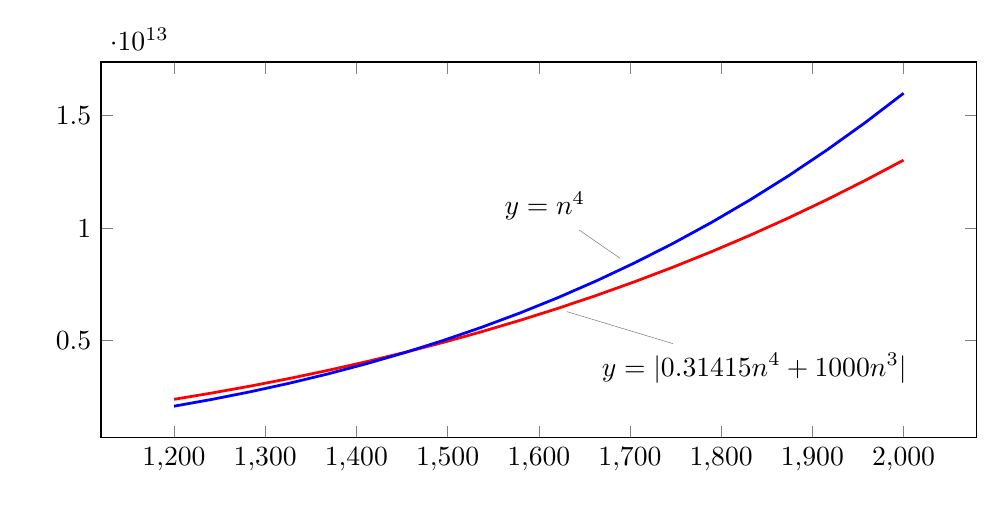
\begin{tikzpicture}[line width=1]
\begin{axis}[width=5in, height=2.5in,
             scatter/classes={a={mark=*,draw=black}},
             xlabel={\mbox{}},
             xlabel style={name=xlabel}, 
             ylabel={\mbox{}}, 
             legend style={
                at={(xlabel.south)},
                yshift=-1ex,
                anchor=north,
                legend cell align=left,
                },
        ]
]
\addplot[draw=red, line width=1] coordinates {(1200.0,2379421440000.0)
(1242.1053,2664126190933.465)
(1284.2105,2972356506808.8804)
(1326.3158,3305271177113.7437)
(1368.4211,3664052688361.816)
(1410.5263,4049907224093.126)
(1452.6316,4464064664873.969)
(1494.7368,4907778588296.902)
(1536.8421,5382326268980.753)
(1578.9474,5889008678570.613)
(1621.0526,6429150485737.84)
(1663.1579,7004100056180.057)
(1705.2632,7615229452621.153)
(1747.3684,8263934434811.285)
(1789.4737,8951634459526.873)
(1831.5789,9679772680570.607)
(1873.6842,10449815948771.436)
(1915.7895,11263254811984.582)
(1957.8947,12121603515091.527)
(2000.0,13026400000000.0)};\node[pin=below right:{$y=|0.31415 n^{4} + 1000n^3|$}] at (axis cs:1620,6415228384344.0) {};\addplot[draw=blue, line width=1] coordinates {(1200.0,2073600000000.0)
(1242.1053,2380310476438.9473)
(1284.2105,2719849675800.5244)
(1326.3158,3094480564145.458)
(1368.4211,3506541539736.499)
(1410.5263,3958446433038.424)
(1452.6316,4452684506718.031)
(1494.7368,4991820455644.1455)
(1536.8421,5578494406887.615)
(1578.9474,6215421919721.3125)
(1621.0526,6905393985620.133)
(1663.1579,7651277028260.998)
(1705.2632,8456012903522.854)
(1747.3684,9322618899486.668)
(1789.4737,10254187736435.436)
(1831.5789,11253887566854.174)
(1873.6842,12324961975429.926)
(1915.7895,13470729979051.754)
(1957.8947,14694586026810.754)
(2000.0,16000000000000.0)};\node[pin=above left:{$y=n^{4}$}] at (axis cs:1700,8352100000000) {};
\end{axis}\end{tikzpicture}\end{center}

he blue graph of $20n^2$ is above the red graph of $f(n)$
on the interval $[10, 10.1]$.
By zooming in at different places on the positive part of the real
axis, we see that the blue graph is always above the red graph.
In fact
\[
|f_0(n)| \leq 20n^2
\]
for all $n > 0$.
This can be proven mathematically:
If $n > 0$, then
\[
n^3 < n^3 + 1
\]
Therefore
\[
\frac{1}{n^3 + 1} < \frac{1}{n^3}
\]
and hence
\[
20 \frac{n^5}{n^3 + 1} < 20 \frac{n^5}{n^3} = 20 n^2
\]
Therefore if we choose $C_0 = 20$ and $N_0 = 1$,
we see that for $n \geq N_0$,
\[
\left|
20 \frac{n^5}{n^3 + 1}
\right| 
\leq C_0
\left|
n^2
\right|
\]
i.e.,
\[
|f_0(n)| \leq C_0|g(n)|
\]
Hence
\[
f_0(n) = O(n^2)
\]

(b)
Let $f_1(n) = 5n^3\cos(n)$.
The following are plots of $|f_1(n)|$ (in red) and $5n^3$:
%-*-latex-*-

\begin{center}
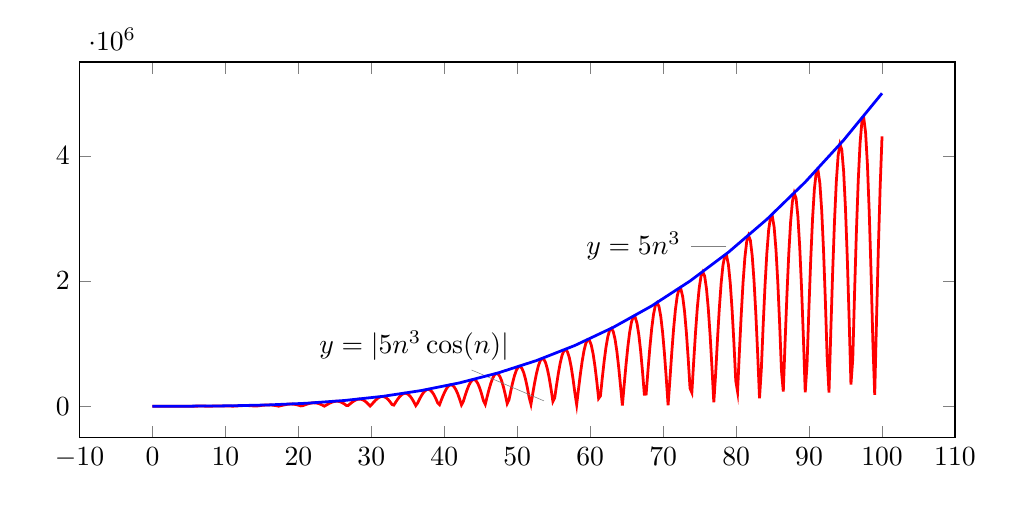
\begin{tikzpicture}[line width=1]
\begin{axis}[width=5in, height=2.5in,
             scatter/classes={a={mark=*,draw=black}},
             xlabel={\mbox{}},
             xlabel style={name=xlabel}, 
             ylabel={\mbox{}}, 
             legend style={
                at={(xlabel.south)},
                yshift=-1ex,
                anchor=north,
                legend cell align=left,
                },
        ]
]
\addplot[draw=red, line width=1] coordinates {(0.0,0.0)
(0.2506,0.0763)
(0.5013,0.5522)
(0.7519,1.5523)
(1.0025,2.7112)
(1.2531,3.0733)
(1.5038,1.1389)
(1.7544,4.9289)
(2.005,16.9548)
(2.2556,36.2973)
(2.5063,63.355)
(2.7569,97.1108)
(3.0075,134.7969)
(3.2581,171.7611)
(3.5088,201.5937)
(3.7594,216.5526)
(4.01,208.2859)
(4.2607,168.8152)
(4.5113,91.7007)
(4.7619,26.7226)
(5.0125,186.178)
(5.2632,381.5007)
(5.5138,602.063)
(5.7644,831.7033)
(6.015,1049.2541)
(6.2657,1229.7156)
(6.5163,1346.0573)
(6.7669,1371.5641)
(7.0175,1282.5724)
(7.2682,1061.3843)
(7.5188,699.0954)
(7.7694,198.0495)
(8.0201,426.3737)
(8.2707,1144.906)
(8.5213,1914.6862)
(8.7719,2680.8415)
(9.0226,3379.3878)
(9.2732,3941.368)
(9.5238,4298.0256)
(9.7744,4386.6931)
(10.0251,4156.9736)
(10.2757,3576.719)
(10.5263,2637.2653)
(10.7769,1357.3907)
(11.0276,214.4926)
(11.2782,2000.3067)
(11.5288,3894.691)
(11.7794,5769.8841)
(12.0301,7482.9906)
(12.2807,8885.308)
(12.5313,9833.1944)
(12.782,10199.7711)
(13.0326,9886.6226)
(13.2832,8834.5691)
(13.5338,7032.569)
(13.7845,4523.8674)
(14.0351,1408.6343)
(14.2857,2157.4582)
(14.5363,5969.008)
(14.787,9780.9831)
(15.0376,13322.7913)
(15.2882,16315.6277)
(15.5388,18492.0937)
(15.7895,19616.822)
(16.0401,19506.6556)
(16.2907,18048.8376)
(16.5414,15215.6878)
(16.792,11074.3758)
(17.0426,5790.6524)
(17.2932,374.2455)
(17.5439,7073.8589)
(17.7945,13893.7811)
(18.0451,20375.2581)
(18.2957,26043.91)
(18.5464,30441.9077)
(18.797,33161.5538)
(19.0476,33877.9669)
(19.2982,32378.4552)
(19.5489,28586.2311)
(19.7995,22576.3511)
(20.0501,14582.1731)
(20.3008,4991.1776)
(20.5514,5670.3211)
(20.802,16763.2878)
(21.0526,27571.8321)
(21.3033,37346.9858)
(21.5539,45355.8698)
(21.8045,50933.1757)
(22.0551,53531.5218)
(22.3058,52767.095)
(22.5564,48457.0873)
(22.807,40645.785)
(23.0576,29616.7626)
(23.3083,15889.4411)
(23.5589,199.251)
(23.8095,16538.266)
(24.0602,33277.9478)
(24.3108,48907.524)
(24.5614,62318.5914)
(24.812,72481.6988)
(25.0627,78520.6432)
(25.3133,79780.8477)
(25.5639,75886.801)
(25.8145,66783.9973)
(26.0652,52761.6217)
(26.3158,34453.3308)
(26.5664,12814.8258)
(26.817,10921.5658)
(27.0677,35313.5094)
(27.3183,58793.1453)
(27.5689,79764.7012)
(27.8195,96709.3532)
(28.0702,108290.6501)
(28.3208,113453.421)
(28.5714,111509.1585)
(28.8221,102201.4189)
(29.0727,85745.8)
(29.3233,62840.4934)
(29.5739,34645.1939)
(29.8246,2728.1651)
(30.0752,31016.6014)
(30.3258,64478.0898)
(30.5764,95456.8453)
(30.8271,121805.8331)
(31.0777,141574.7699)
(31.3283,153148.4713)
(31.5789,155369.7079)
(31.8296,147637.6489)
(32.0802,129974.1848)
(32.3308,103052.2069)
(32.5815,68182.1851)
(32.8321,27256.0026)
(33.0827,17350.1992)
(33.3333,62909.5949)
(33.584,106507.4766)
(33.8346,145223.8187)
(34.0852,176324.4133)
(34.3358,197448.3196)
(34.5865,206779.0794)
(34.8371,203187.6808)
(35.0877,186336.6092)
(35.3383,156736.441)
(35.589,115749.2164)
(35.8396,65536.1026)
(36.0902,8950.4362)
(36.3409,50619.1093)
(36.5915,109446.9991)
(36.8421,163699.6336)
(37.0927,209680.6848)
(37.3434,244077.5372)
(37.594,264192.7061)
(37.8446,268144.4457)
(38.0952,255022.1602)
(38.3459,224984.6319)
(38.5965,179292.3703)
(38.8471,120269.3725)
(39.0977,51194.0407)
(39.3484,23876.3609)
(39.599,100338.794)
(39.8496,173322.0555)
(40.1003,237992.4668)
(40.3509,289868.748)
(40.6015,325125.8696)
(40.8521,340867.646)
(41.1028,335349.1288)
(41.3534,308132.449)
(41.604,260163.5052)
(41.8546,193761.6128)
(42.1053,112519.6283)
(42.3559,21117.8178)
(42.6065,74939.5124)
(42.8571,169650.2485)
(43.1078,256884.582)
(43.3584,330776.4936)
(43.609,386111.9194)
(43.8596,418688.2714)
(44.1103,425620.9749)
(44.3609,405575.2984)
(44.6115,358905.8734)
(44.8622,287691.7059)
(45.1128,195660.8683)
(45.3634,88006.0344)
(45.614,28900.8461)
(45.8647,147879.6108)
(46.1153,261377.4951)
(46.3659,361943.2114)
(46.6165,442710.0727)
(46.8672,497857.1899)
(47.1178,523018.1948)
(47.3684,515609.3588)
(47.619,475053.3051)
(47.8697,402880.5146)
(48.1203,302698.1859)
(48.3709,180024.2655)
(48.6216,41993.1279)
(48.8722,103052.1033)
(49.1228,246057.8051)
(49.3734,377819.3212)
(49.6241,489567.4324)
(49.8747,573544.8237)
(50.1253,623535.0658)
(50.3759,635308.5597)
(50.6266,606954.1891)
(50.8772,539071.8708)
(51.1278,434809.4348)
(51.3784,299736.827)
(51.6291,141560.917)
(51.8797,30305.4222)
(52.1303,205296.4948)
(52.381,372337.187)
(52.6316,520537.8134)
(52.8822,639897.1873)
(53.1328,721968.9271)
(53.3835,760447.095)
(53.6341,751631.2117)
(53.8847,694737.3315)
(54.1353,592030.8359)
(54.386,448767.4013)
(54.6366,272940.5637)
(54.8872,74846.7108)
(55.1378,133509.6229)
(55.3885,339136.3801)
(55.6391,528857.7163)
(55.8897,690151.5318)
(56.1404,811967.9669)
(56.391,885475.8259)
(56.6416,904687.0969)
(56.8922,866916.2323)
(57.1429,773040.3147)
(57.3935,627538.1223)
(57.6441,438299.7268)
(57.8947,216212.7688)
(58.1454,25453.9409)
(58.396,271835.3033)
(58.6466,507377.3956)
(58.8972,716812.5697)
(59.1479,886141.4742)
(59.3985,1003559.2899)
(59.6491,1060265.4407)
(59.8997,1051101.9679)
(60.1504,974975.352)
(60.401,835029.3033)
(60.6516,638551.1912)
(60.9023,396611.4146)
(61.1529,123452.1111)
(61.4035,164341.9299)
(61.6541,448842.5241)
(61.9048,711887.8159)
(62.1554,936234.2321)
(62.406,1106678.052)
(62.6566,1211074.1597)
(62.9073,1241184.3701)
(63.1579,1193296.9908)
(63.4085,1068572.5221)
(63.6591,873086.8336)
(63.9098,617561.8292)
(64.1604,316793.3621)
(64.411,11194.2446)
(64.6617,346219.5402)
(64.9123,667178.0623)
(65.1629,953364.2542)
(65.4135,1185798.8498)
(65.6642,1348477.1312)
(65.9148,1429456.5625)
(66.1654,1421710.6881)
(66.416,1323689.4369)
(66.6667,1139543.3615)
(66.9173,878989.8374)
(67.1679,556821.6148)
(67.4185,192080.9649)
(67.6692,193055.4633)
(67.9198,574616.4759)
(68.1704,928320.4692)
(68.4211,1231112.4755)
(68.6717,1462657.3234)
(68.9223,1606692.7727)
(69.1729,1652153.2995)
(69.4236,1593987.8781)
(69.6742,1433612.9482)
(69.9248,1178963.7424)
(70.1754,844131.9674)
(70.4261,448603.949)
(70.6767,16139.1327)
(70.9273,426647.3777)
(71.1779,851914.3326)
(71.4286,1232336.6759)
(71.6792,1542852.1878)
(71.9298,1762301.3292)
(72.1805,1874853.6486)
(72.4311,1871125.4624)
(72.6817,1748911.195)
(72.9323,1513473.7512)
(73.183,1177366.2492)
(73.4336,759786.7135)
(73.6842,285497.111)
(73.9348,216633.5004)
(74.1855,715376.774)
(74.4361,1179078.6247)
(74.6867,1577659.356)
(74.9373,1884554.5221)
(75.188,2078471.9108)
(75.4386,2144849.2127)
(75.6892,2076913.6687)
(75.9398,1876268.3342)
(76.1905,1552958.2131)
(76.4411,1125001.6754)
(76.6917,617406.3008)
(76.9424,60721.4716)
(77.193,510789.465)
(77.4436,1061248.8147)
(77.6942,1555407.8683)
(77.9449,1960894.235)
(78.1955,2250320.4909)
(78.4461,2403117.4955)
(78.6967,2406970.593)
(78.9474,2258759.8051)
(79.198,1964934.7538)
(79.4486,1541289.65)
(79.6992,1012141.1556)
(79.9499,408949.9283)
(80.2005,231537.2119)
(80.4511,869515.6361)
(80.7018,1464587.3219)
(80.9524,1978309.3446)
(81.203,2376666.261)
(81.4536,2632308.0441)
(81.7043,2726407.1605)
(81.9549,2650009.8552)
(82.2055,2404786.5133)
(82.4561,2003122.3726)
(82.7068,1467530.671)
(82.9574,829413.0054)
(83.208,127233.583)
(83.4586,595787.5271)
(83.7093,1294324.5806)
(83.9599,1923777.9257)
(84.2105,2443111.0391)
(84.4612,2817512.9997)
(84.7118,3020714.4163)
(84.9624,3036803.7337)
(85.213,2861419.8088)
(85.4637,2502234.0176)
(85.7143,1978678.6913)
(85.9649,1320925.7325)
(86.2155,568166.9033)
(86.4662,233707.5135)
(86.7168,1034895.1159)
(86.9674,1784764.3895)
(87.218,2435044.1068)
(87.4687,2942918.8433)
(87.7193,3273832.8138)
(87.9699,3403819.3008)
(88.2206,3321199.8759)
(88.4712,3027534.8962)
(88.7218,2537752.1905)
(88.9724,1879431.7083)
(89.2231,1091277.0332)
(89.4737,220856.736)
(89.7243,678253.7596)
(89.9749,1549758.918)
(90.2256,2338157.5019)
(90.4762,2992265.9065)
(90.7268,3468527.4297)
(90.9774,3733894.3274)
(91.2281,3768093.012)
(91.4787,3565118.6879)
(91.7293,3133851.9849)
(91.9799,2497744.0077)
(92.2306,1693574.3504)
(92.4812,769345.4349)
(92.7318,218567.7153)
(92.9825,1208844.0401)
(93.2331,2139011.861)
(93.4837,2949378.929)
(93.7343,3586850.5417)
(93.985,4008392.2666)
(94.2356,4183912.3777)
(94.4862,4098372.2365)
(94.7368,3752978.6583)
(94.9875,3165368.0881)
(95.2381,2368754.8128)
(95.4887,1410080.5783)
(95.7393,347266.8011)
(95.99,754271.0185)
(96.2406,1825637.8429)
(96.4912,2798756.9837)
(96.7419,3610683.9097)
(96.9925,4207663.3489)
(97.2431,4548669.0396)
(97.4937,4608194.1568)
(97.7444,4378104.2511)
(97.995,3868420.9424)
(98.2456,3106970.2332)
(98.4962,2137900.1305)
(98.7469,1019143.8833)
(98.9975,181026.9677)
(99.2481,1388155.7341)
(99.4987,2526208.1198)
(99.7494,3522349.7702)
(100.0,4311594.3614)};\node[pin=above left:{$y=|5n^3 \cos(n)|$}] at (axis cs:55,18406.695365414427) {};\addplot[draw=blue, line width=1] coordinates {(0.0,0.0)
(5.2632,728.9692)
(10.5263,5831.7539)
(15.7895,19682.1694)
(21.0526,46654.0312)
(26.3158,91121.1547)
(31.5789,157457.3553)
(36.8421,250036.4485)
(42.1053,373232.2496)
(47.3684,531418.5741)
(52.6316,728969.2375)
(57.8947,970258.0551)
(63.1579,1259658.8424)
(68.4211,1601545.4148)
(73.6842,2000291.5877)
(78.9474,2460271.1766)
(84.2105,2985857.9968)
(89.4737,3581425.8638)
(94.7368,4251348.5931)
(100.0,5000000.0)};\node[pin=left:{$y=5n^3$}] at (axis cs:80,2560000) {};
\end{axis}\end{tikzpicture}\end{center}

Since
\[
-1 \leq \cos(n) \leq 1
\]
for $n \geq 0$, we have
\[
-5n^3 \leq 5n^3 \cos(n) \leq 5n^3
\]
Therefore
\[
|5n^3 \cos(n)| \leq 5|n^3|
\]
Hence if I can choose $C_1 = 5$, $N_1 = 0$,
then for $n \geq N_1$,
\[
|5n^3 \cos(n)| \leq 5|n^3|
\]
i.e.,
\[
|f_1(n)| \leq 5|n^3|
\]
Therefore
\[
f_1(n) = O(5n^3)
\]

(c)
Let $f_2(n) = 7^8$.
The following are plots of $|f_2(n)|$ (in red) and $7^8n^0$:
%-*-latex-*-

\begin{center}
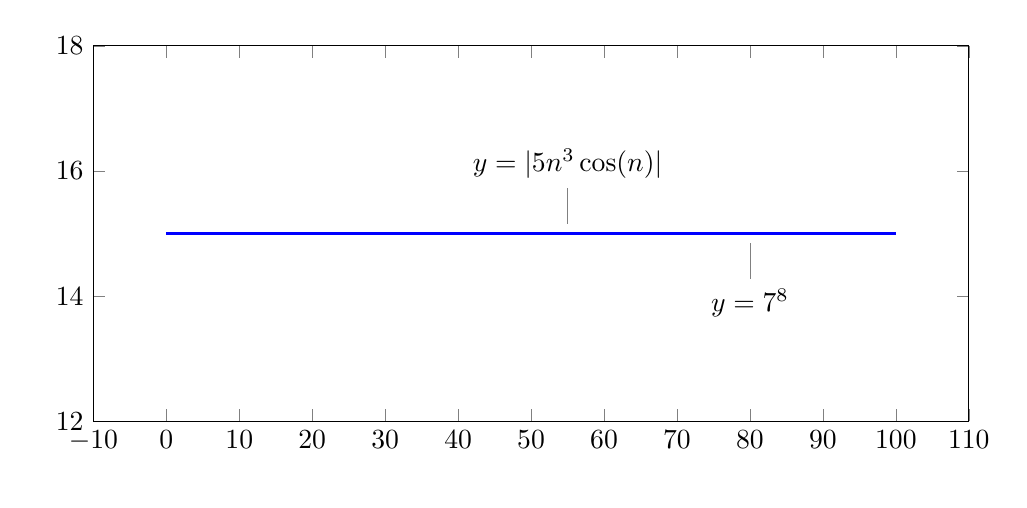
\begin{tikzpicture}[line width=1]
\begin{axis}[width=5in, height=2.5in,
             scatter/classes={a={mark=*,draw=black}},
             xlabel={\mbox{}},
             xlabel style={name=xlabel}, 
             ylabel={\mbox{}}, 
             legend style={
                at={(xlabel.south)},
                yshift=-1ex,
                anchor=north,
                legend cell align=left,
                },
        ]
]
\addplot[draw=red, line width=1] coordinates {(0.0,15)
(50.0,15)
(100.0,15)
(100.0,15)};\node[pin=above:{$y=|5n^3 \cos(n)|$}] at (axis cs:55,15) {};\addplot[draw=blue, line width=1] coordinates {(0.0,15)
(50.0,15)
(100.0,15)
(100.0,15)};\node[pin=below:{$y=7^8$}] at (axis cs:80,15) {};
\end{axis}\end{tikzpicture}\end{center}

The two graphs are the same.
If I set $C_2 = 7^8$ and $N_2 = 0$, then for $n \geq N_2$,
\[
|f_2(n)| \leq C_2|n^0|
\]
Therefore
\[
f_2(n) = O(n^0)
\]

(d) Let $C = \max(C_0, C_1, C_2) = \max(20, 5, 7^8) = 7^8$,
$N = \max(N_0, N_1, N_2) = \max(1, 0, 0) = 1$,
$k = \max(2, 3, 0) = 3$.

%-*-latex-*-

\begin{center}
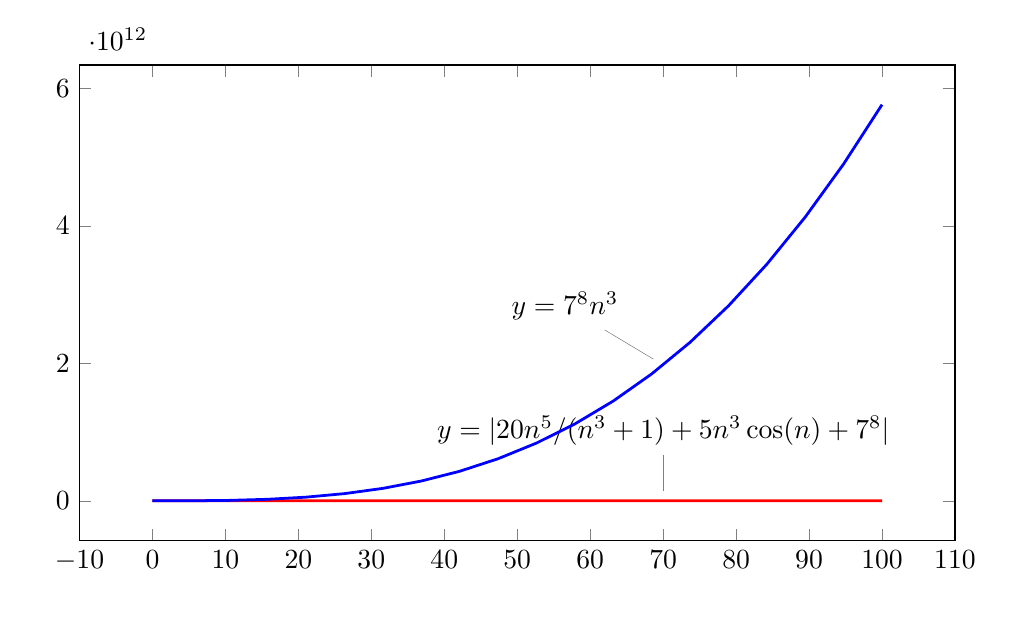
\begin{tikzpicture}[line width=1]
\begin{axis}[width=5in, height=3in,
             scatter/classes={a={mark=*,draw=black}},
             xlabel={\mbox{}},
             xlabel style={name=xlabel}, 
             ylabel={\mbox{}}, 
             legend style={
                at={(xlabel.south)},
                yshift=-1ex,
                anchor=north,
                legend cell align=left,
                },
        ]
]
\addplot[draw=red, line width=1] coordinates {(0.0,5764801.0)
(0.2506,5764801.0957)
(0.5013,5764802.1143)
(0.7519,5764805.9247)
(1.0025,5764813.7992)
(1.2531,5764824.8977)
(1.5038,5764837.0872)
(1.7544,5764848.0098)
(2.005,5764855.5726)
(2.2556,5764858.3048)
(2.5063,5764855.7689)
(2.7569,5764848.9742)
(3.0075,5764840.6923)
(3.2581,5764835.5831)
(3.5088,5764840.0649)
(3.7594,5764861.8872)
(4.01,5764909.4088)
(4.2607,5764990.6137)
(4.5113,5765111.9463)
(4.7619,5765277.0759)
(5.0125,5765485.7288)
(5.2632,5765732.7432)
(5.5138,5766007.4936)
(5.7644,5766293.8204)
(6.015,5766570.5579)
(6.2657,5766812.7075)
(6.5163,5766993.24)
(6.7669,5767085.4414)
(7.0175,5767065.6491)
(7.2682,5766916.1658)
(7.5188,5766628.0878)
(7.7694,5766203.7597)
(8.0201,5765658.5614)
(8.2707,5765021.762)
(8.5213,5764336.2227)
(8.7719,5763656.817)
(9.0226,5763047.529)
(9.2732,5762577.3164)
(9.5238,5762314.9358)
(9.7744,5762323.055)
(10.0251,5762652.071)
(10.2757,5763334.1323)
(10.5263,5764377.9028)
(10.7769,5765764.6047)
(11.0276,5767445.8259)
(11.2782,5769343.4885)
(11.5288,5771352.2321)
(11.7794,5773344.2955)
(12.0301,5775176.7832)
(12.2807,5776700.9931)
(12.5313,5777773.283)
(12.782,5778266.7746)
(13.0326,5778083.0523)
(13.2832,5777162.9364)
(13.5338,5775495.3854)
(13.7845,5773123.6444)
(14.0351,5770147.8835)
(14.2857,5766723.7749)
(14.5363,5763056.7207)
(14.787,5759391.7529)
(15.0376,5755999.4638)
(15.2882,5753158.6582)
(15.5388,5751136.735)
(15.7895,5750169.0613)
(16.0401,5750438.7942)
(16.2907,5752058.6906)
(16.5414,5755056.4308)
(16.792,5759364.8452)
(17.0426,5764818.1831)
(17.2932,5771155.2074)
(17.5439,5778029.4593)
(17.7945,5785026.5322)
(18.0451,5791687.6718)
(18.2957,5797538.4986)
(18.5464,5802121.1832)
(18.797,5805028.0285)
(19.0476,5805934.1529)
(19.2982,5804626.8647)
(19.5489,5801029.3762)
(19.7995,5795216.7441)
(20.0501,5787422.3263)
(20.3008,5778033.6031)
(20.5514,5767576.889)
(20.802,5756691.2192)
(21.0526,5746092.484)
(21.3033,5736529.6516)
(21.5539,5728735.6013)
(21.8045,5723375.6414)
(22.0551,5720997.1536)
(22.3058,5721983.951)
(22.5564,5726518.8415)
(22.807,5734557.5391)
(23.0576,5745816.4691)
(23.3083,5759776.2106)
(23.5589,5775701.3329)
(23.8095,5792676.2945)
(24.0602,5809655.9334)
(24.3108,5825527.9789)
(24.5614,5839184.028)
(24.812,5849594.6296)
(25.0627,5855883.5804)
(25.3133,5857396.3038)
(25.5639,5853757.2884)
(25.8145,5844912.0283)
(26.0652,5831149.7088)
(26.3158,5813103.9863)
(26.5664,5791730.5622)
(26.817,5768261.7639)
(27.0677,5744139.9261)
(27.3183,5720932.9083)
(27.5689,5700236.483)
(27.8195,5683569.4739)
(28.0702,5672268.3325)
(28.3208,5667388.2294)
(28.5714,5669617.6721)
(28.8221,5679213.1044)
(29.0727,5695958.9286)
(29.3233,5719156.9527)
(29.5739,5747647.4823)
(29.8246,5779862.2536)
(30.0752,5813907.2751)
(30.3258,5847671.5309)
(30.5764,5878955.5662)
(30.8271,5905612.3464)
(31.0777,5925691.588)
(31.3283,5937578.1066)
(31.5789,5940114.6729)
(31.8296,5932700.4561)
(32.0802,5915357.3467)
(32.3308,5888758.2359)
(32.5815,5854213.5937)
(32.8321,5813615.3032)
(33.0827,5769339.506)
(33.3333,5724113.0273)
(33.584,5680850.5751)
(33.8346,5642472.175)
(34.0852,5611712.0349)
(34.3358,5590931.0955)
(34.5865,5581945.8152)
(34.8371,5585885.2057)
(35.0877,5603086.7817)
(35.3383,5633039.9669)
(35.589,5674382.7208)
(35.8396,5724953.8765)
(36.0902,5781900.0972)
(36.3409,5841832.7097)
(36.5915,5901026.1788)
(36.8421,5955646.9052)
(37.0927,6001998.5607)
(37.3434,6036768.53)
(37.594,6057259.3282)
(37.8446,6061589.2097)
(38.0952,6048847.5785)
(38.3459,6019193.2171)
(38.5965,5973886.6348)
(38.8471,5915251.8289)
(39.0977,5846567.2014)
(39.3484,5771890.0168)
(39.599,5695823.313)
(39.8496,5623238.2934)
(40.1003,5558968.6365)
(40.3509,5507495.6222)
(40.6015,5472644.2799)
(40.8521,5457310.7955)
(41.1028,5463240.1171)
(41.3534,5490870.1139)
(41.604,5539254.8871)
(41.8546,5606075.1214)
(42.1053,5687737.9604)
(42.3559,5779563.138)
(42.6065,5876046.3477)
(42.8571,5971185.4757)
(43.1078,6058850.7137)
(43.3584,6133176.0424)
(43.609,6188947.3977)
(43.8596,6221962.1918)
(44.1103,6229335.8499)
(44.3609,6209733.6405)
(44.6115,6163510.1952)
(44.8622,6092744.5198)
(45.1128,6001164.6869)
(45.3634,5893963.3702)
(45.614,5777512.5194)
(45.8647,5658992.2969)
(46.1153,5545955.4674)
(46.3659,5445853.3183)
(46.6165,5365552.5368)
(46.8672,5310874.0119)
(47.1178,5286184.1119)
(47.3684,5294066.5652)
(47.619,5335098.7489)
(47.8697,5407750.1818)
(48.1203,5508413.6654)
(48.3709,5631571.2533)
(48.6216,5770088.5708)
(48.8722,5915622.4945)
(49.1228,6059119.4013)
(49.3734,6191374.635)
(49.6241,6303618.9763)
(49.8747,6388095.1102)
(50.1253,6438586.6074)
(50.3759,6450863.869)
(50.6266,6423015.7786)
(50.8772,6355642.253)
(51.1278,6251891.1222)
(51.3784,6117332.3322)
(51.6291,5959672.7526)
(51.8797,5788325.2562)
(52.1303,5613855.5389)
(52.381,5447338.7146)
(52.6316,5299664.4686)
(52.8822,5180833.9877)
(53.1328,5099293.6534)
(53.3835,5061349.4035)
(53.6341,5070701.7173)
(53.8847,5128134.5407)
(54.1353,5231382.4918)
(54.386,5375189.8945)
(54.6366,5551563.2129)
(54.8872,5750206.0589)
(55.1378,5959113.8984)
(55.3885,6165294.6738)
(55.6391,6355572.5408)
(55.8897,6517425.3997)
(56.1404,6639803.3906)
(56.391,6713875.318)
(56.6416,6733653.1699)
(56.8922,6696451.3988)
(57.1429,6603147.0871)
(57.3935,6458219.0133)
(57.6441,6269557.2488)
(57.8947,6048049.4345)
(58.1454,5806964.3808)
(58.396,5561167.1871)
(58.6466,5326211.776)
(58.8972,5117365.7957)
(59.1479,4948628.5974)
(59.3985,4831805.0005)
(59.6491,4775695.5811)
(59.8997,4785458.2977)
(60.1504,4862186.67)
(60.401,5002736.9877)
(60.6516,5199821.8812)
(60.9023,5442370.9519)
(61.1529,5716142.0618)
(61.4035,6004550.422)
(61.6541,6289667.8478)
(61.9048,6553332.4837)
(62.1554,6778300.7567)
(62.406,6949368.9458)
(62.6566,7054391.9353)
(62.9073,7085131.5399)
(63.1579,7037876.0675)
(63.4085,6913786.0182)
(63.6591,6718937.2616)
(63.9098,6464051.7016)
(64.1604,6163925.1915)
(64.411,5836582.0544)
(64.6617,5502203.7408)
(64.9123,5181894.7133)
(65.1629,4896360.5285)
(65.4135,4664580.4526)
(65.6642,4502559.2035)
(65.9148,4422239.3169)
(66.1654,4430647.2486)
(66.416,4529333.0696)
(66.6667,4714146.2274)
(66.9173,4975369.3464)
(67.1679,5298209.6764)
(67.4185,5663624.9463)
(67.6692,6049438.507)
(67.9198,6431679.1647)
(68.1704,6786065.3156)
(68.4211,7089541.992)
(68.6717,7321774.0227)
(68.9223,7466499.1672)
(69.1729,7512651.9017)
(69.4236,7455181.2006)
(69.6742,7295503.5035)
(69.9248,7041554.0431)
(70.1754,6707424.5261)
(70.4261,6312601.2781)
(70.6767,5880843.7448)
(70.9273,5438767.0299)
(71.1779,5014212.3831)
(71.4286,4634504.8604)
(71.6792,4324706.6817)
(71.9298,4105977.386)
(72.1805,3994147.4249)
(72.4311,3998600.4818)
(72.6817,4121542.1325)
(72.9323,4357709.4721)
(73.183,4694549.3826)
(73.4336,5112863.8392)
(73.6842,5587890.8752)
(73.9348,6090761.4326)
(74.1855,6590247.1647)
(74.4361,7054693.9866)
(74.6867,7454022.2015)
(74.9373,7761667.3638)
(75.188,7956337.2612)
(75.4386,8023469.5844)
(75.6892,7956291.5742)
(75.9398,7756406.286)
(76.1905,7433858.7239)
(76.4411,7006667.2576)
(76.6917,6499839.4669)
(76.9424,5943924.7342)
(77.193,5373186.4068)
(77.4436,4823502.1786)
(77.6942,4330120.7592)
(77.9449,3925414.5392)
(78.1955,3636770.9425)
(78.4461,3484759.1096)
(78.6967,3481693.6964)
(78.9474,3630694.6812)
(79.198,3925312.4418)
(79.4486,4349752.7676)
(79.6992,4879698.9965)
(79.9499,5483690.4708)
(80.2005,6124980.3706)
(80.4511,6763764.0669)
(80.7018,7359643.5373)
(80.9524,7874175.8571)
(81.203,8273345.5833)
(81.4536,8529802.6887)
(81.7043,8624719.6399)
(81.9549,8549142.6819)
(82.2055,8304742.1999)
(82.4561,7903903.4317)
(82.7068,7369139.615)
(82.9574,6731852.347)
(83.208,6030505.8347)
(83.4586,5308320.1471)
(83.7093,4610621.0288)
(83.9599,3982008.1314)
(84.2105,3463517.9783)
(84.4612,3089961.4905)
(84.7118,2887608.0591)
(84.9624,2872369.2396)
(85.213,3048606.175)
(85.4637,3408647.4891)
(85.7143,3933060.8509)
(85.9649,4591674.3577)
(86.2155,5345296.2475)
(86.4662,6148036.2374)
(86.7168,6950091.9255)
(86.9674,7700831.7973)
(87.218,8351984.6253)
(87.4687,8860734.9851)
(87.7193,9192527.0915)
(87.9699,9323394.2268)
(88.2206,9241657.9629)
(88.4712,8948878.6567)
(88.7218,8459984.137)
(88.9724,7802554.3534)
(89.2231,7015292.8893)
(89.4737,6145768.3158)
(89.7243,5247556.0564)
(89.9749,4376951.6467)
(90.2256,3589456.324)
(90.4762,2936253.6933)
(90.7268,2460900.4564)
(90.9774,2196444.3577)
(91.2281,2163158.9845)
(91.4787,2367049.1326)
(91.7293,2799234.1721)
(91.9799,3436262.9984)
(92.2306,4241356.0174)
(92.4812,5166510.807)
(92.7318,6155352.344)
(92.9825,7146559.568)
(93.2331,8077660.8007)
(93.4837,8888963.793)
(93.7343,9527373.8426)
(93.985,9949856.517)
(94.2356,10126320.09)
(94.4862,10041725.9234)
(94.7368,9697280.8322)
(94.9875,9110621.2616)
(95.2381,8314961.4985)
(95.4887,7357243.2887)
(95.7393,6295388.0488)
(95.99,5194811.2789)
(96.2406,4124408.0168)
(96.4912,3152254.9509)
(96.7419,2341296.6123)
(96.9925,1745288.2731)
(97.2431,1405256.1949)
(97.4937,1346707.2028)
(97.7444,1577775.7461)
(97.995,2088440.2049)
(98.2456,2850874.5767)
(98.4962,3820930.8547)
(98.7469,4940675.7897)
(98.9975,6141837.841)
(99.2481,7349960.3203)
(99.4987,8489008.9313)
(99.7494,9486149.3197)
(100.0,10276395.1614)};\node[pin=above:{$y=|20n^5 /(n^3 + 1) + 5n^3 \cos(n) + 7^8|$}] at (axis cs:70,6948943.147579552) {};\addplot[draw=blue, line width=1] coordinates {(0.0,0.0)
(5.2632,840472517.8597)
(10.5263,6723780142.878)
(15.7895,22692757982.2132)
(21.0526,53790241143.0238)
(26.3158,105059064732.4683)
(31.5789,181542063857.7052)
(36.8421,288282073625.8931)
(42.1053,430321929144.1902)
(47.3684,612704465519.7552)
(52.6316,840472517859.7465)
(57.8947,1118668921271.3225)
(63.1579,1452336510861.6418)
(68.4211,1846518121737.8638)
(73.6842,2306256589007.146)
(78.9474,2836594747776.6465)
(84.2105,3442575433153.525)
(89.4737,4129241480244.9395)
(94.7368,4901635724158.049)
(100.0,5764801000000.0)};\node[pin=above left:{$y=7^8 n^3$}] at (axis cs:70,1977326743000) {};
\end{axis}\end{tikzpicture}\end{center}

No. $f(n)$ is not flat.
It appears to be flat only because $7^8n^3$ is climbing too fast.
Here's the plot of $f(n)$ without $7^8n^3$

\begin{center}
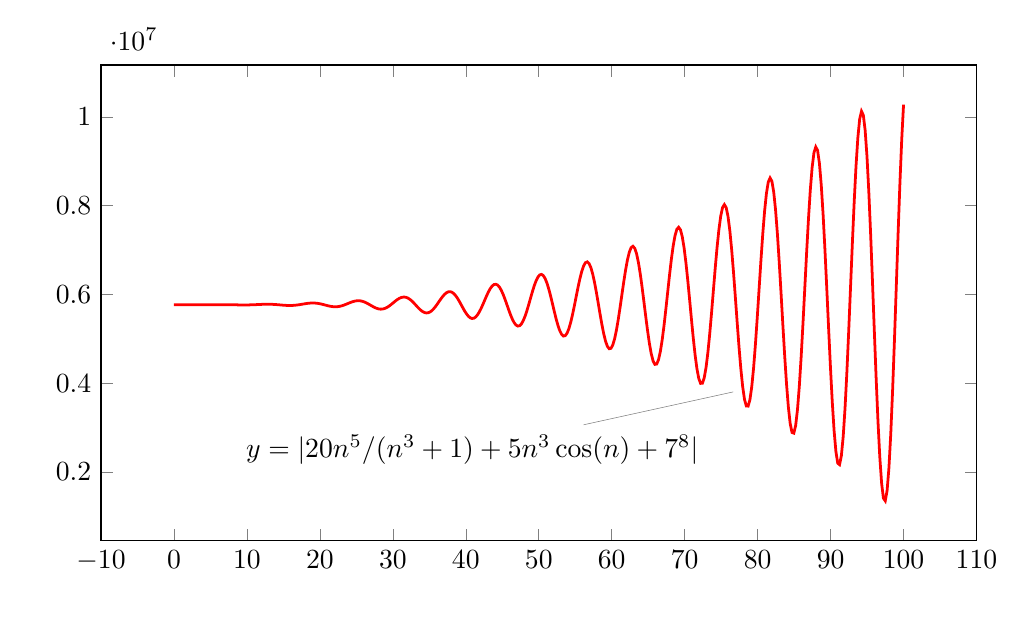
\begin{tikzpicture}[line width=1]
\begin{axis}[width=5in, height=3in,
             scatter/classes={a={mark=*,draw=black}},
             xlabel={\mbox{}},
             xlabel style={name=xlabel}, 
             ylabel={\mbox{}}, 
             legend style={
                at={(xlabel.south)},
                yshift=-1ex,
                anchor=north,
                legend cell align=left,
                },
        ]
]
\addplot[draw=red, line width=1] coordinates {(0.0,5764801.0)
(0.2506,5764801.0957)
(0.5013,5764802.1143)
(0.7519,5764805.9247)
(1.0025,5764813.7992)
(1.2531,5764824.8977)
(1.5038,5764837.0872)
(1.7544,5764848.0098)
(2.005,5764855.5726)
(2.2556,5764858.3048)
(2.5063,5764855.7689)
(2.7569,5764848.9742)
(3.0075,5764840.6923)
(3.2581,5764835.5831)
(3.5088,5764840.0649)
(3.7594,5764861.8872)
(4.01,5764909.4088)
(4.2607,5764990.6137)
(4.5113,5765111.9463)
(4.7619,5765277.0759)
(5.0125,5765485.7288)
(5.2632,5765732.7432)
(5.5138,5766007.4936)
(5.7644,5766293.8204)
(6.015,5766570.5579)
(6.2657,5766812.7075)
(6.5163,5766993.24)
(6.7669,5767085.4414)
(7.0175,5767065.6491)
(7.2682,5766916.1658)
(7.5188,5766628.0878)
(7.7694,5766203.7597)
(8.0201,5765658.5614)
(8.2707,5765021.762)
(8.5213,5764336.2227)
(8.7719,5763656.817)
(9.0226,5763047.529)
(9.2732,5762577.3164)
(9.5238,5762314.9358)
(9.7744,5762323.055)
(10.0251,5762652.071)
(10.2757,5763334.1323)
(10.5263,5764377.9028)
(10.7769,5765764.6047)
(11.0276,5767445.8259)
(11.2782,5769343.4885)
(11.5288,5771352.2321)
(11.7794,5773344.2955)
(12.0301,5775176.7832)
(12.2807,5776700.9931)
(12.5313,5777773.283)
(12.782,5778266.7746)
(13.0326,5778083.0523)
(13.2832,5777162.9364)
(13.5338,5775495.3854)
(13.7845,5773123.6444)
(14.0351,5770147.8835)
(14.2857,5766723.7749)
(14.5363,5763056.7207)
(14.787,5759391.7529)
(15.0376,5755999.4638)
(15.2882,5753158.6582)
(15.5388,5751136.735)
(15.7895,5750169.0613)
(16.0401,5750438.7942)
(16.2907,5752058.6906)
(16.5414,5755056.4308)
(16.792,5759364.8452)
(17.0426,5764818.1831)
(17.2932,5771155.2074)
(17.5439,5778029.4593)
(17.7945,5785026.5322)
(18.0451,5791687.6718)
(18.2957,5797538.4986)
(18.5464,5802121.1832)
(18.797,5805028.0285)
(19.0476,5805934.1529)
(19.2982,5804626.8647)
(19.5489,5801029.3762)
(19.7995,5795216.7441)
(20.0501,5787422.3263)
(20.3008,5778033.6031)
(20.5514,5767576.889)
(20.802,5756691.2192)
(21.0526,5746092.484)
(21.3033,5736529.6516)
(21.5539,5728735.6013)
(21.8045,5723375.6414)
(22.0551,5720997.1536)
(22.3058,5721983.951)
(22.5564,5726518.8415)
(22.807,5734557.5391)
(23.0576,5745816.4691)
(23.3083,5759776.2106)
(23.5589,5775701.3329)
(23.8095,5792676.2945)
(24.0602,5809655.9334)
(24.3108,5825527.9789)
(24.5614,5839184.028)
(24.812,5849594.6296)
(25.0627,5855883.5804)
(25.3133,5857396.3038)
(25.5639,5853757.2884)
(25.8145,5844912.0283)
(26.0652,5831149.7088)
(26.3158,5813103.9863)
(26.5664,5791730.5622)
(26.817,5768261.7639)
(27.0677,5744139.9261)
(27.3183,5720932.9083)
(27.5689,5700236.483)
(27.8195,5683569.4739)
(28.0702,5672268.3325)
(28.3208,5667388.2294)
(28.5714,5669617.6721)
(28.8221,5679213.1044)
(29.0727,5695958.9286)
(29.3233,5719156.9527)
(29.5739,5747647.4823)
(29.8246,5779862.2536)
(30.0752,5813907.2751)
(30.3258,5847671.5309)
(30.5764,5878955.5662)
(30.8271,5905612.3464)
(31.0777,5925691.588)
(31.3283,5937578.1066)
(31.5789,5940114.6729)
(31.8296,5932700.4561)
(32.0802,5915357.3467)
(32.3308,5888758.2359)
(32.5815,5854213.5937)
(32.8321,5813615.3032)
(33.0827,5769339.506)
(33.3333,5724113.0273)
(33.584,5680850.5751)
(33.8346,5642472.175)
(34.0852,5611712.0349)
(34.3358,5590931.0955)
(34.5865,5581945.8152)
(34.8371,5585885.2057)
(35.0877,5603086.7817)
(35.3383,5633039.9669)
(35.589,5674382.7208)
(35.8396,5724953.8765)
(36.0902,5781900.0972)
(36.3409,5841832.7097)
(36.5915,5901026.1788)
(36.8421,5955646.9052)
(37.0927,6001998.5607)
(37.3434,6036768.53)
(37.594,6057259.3282)
(37.8446,6061589.2097)
(38.0952,6048847.5785)
(38.3459,6019193.2171)
(38.5965,5973886.6348)
(38.8471,5915251.8289)
(39.0977,5846567.2014)
(39.3484,5771890.0168)
(39.599,5695823.313)
(39.8496,5623238.2934)
(40.1003,5558968.6365)
(40.3509,5507495.6222)
(40.6015,5472644.2799)
(40.8521,5457310.7955)
(41.1028,5463240.1171)
(41.3534,5490870.1139)
(41.604,5539254.8871)
(41.8546,5606075.1214)
(42.1053,5687737.9604)
(42.3559,5779563.138)
(42.6065,5876046.3477)
(42.8571,5971185.4757)
(43.1078,6058850.7137)
(43.3584,6133176.0424)
(43.609,6188947.3977)
(43.8596,6221962.1918)
(44.1103,6229335.8499)
(44.3609,6209733.6405)
(44.6115,6163510.1952)
(44.8622,6092744.5198)
(45.1128,6001164.6869)
(45.3634,5893963.3702)
(45.614,5777512.5194)
(45.8647,5658992.2969)
(46.1153,5545955.4674)
(46.3659,5445853.3183)
(46.6165,5365552.5368)
(46.8672,5310874.0119)
(47.1178,5286184.1119)
(47.3684,5294066.5652)
(47.619,5335098.7489)
(47.8697,5407750.1818)
(48.1203,5508413.6654)
(48.3709,5631571.2533)
(48.6216,5770088.5708)
(48.8722,5915622.4945)
(49.1228,6059119.4013)
(49.3734,6191374.635)
(49.6241,6303618.9763)
(49.8747,6388095.1102)
(50.1253,6438586.6074)
(50.3759,6450863.869)
(50.6266,6423015.7786)
(50.8772,6355642.253)
(51.1278,6251891.1222)
(51.3784,6117332.3322)
(51.6291,5959672.7526)
(51.8797,5788325.2562)
(52.1303,5613855.5389)
(52.381,5447338.7146)
(52.6316,5299664.4686)
(52.8822,5180833.9877)
(53.1328,5099293.6534)
(53.3835,5061349.4035)
(53.6341,5070701.7173)
(53.8847,5128134.5407)
(54.1353,5231382.4918)
(54.386,5375189.8945)
(54.6366,5551563.2129)
(54.8872,5750206.0589)
(55.1378,5959113.8984)
(55.3885,6165294.6738)
(55.6391,6355572.5408)
(55.8897,6517425.3997)
(56.1404,6639803.3906)
(56.391,6713875.318)
(56.6416,6733653.1699)
(56.8922,6696451.3988)
(57.1429,6603147.0871)
(57.3935,6458219.0133)
(57.6441,6269557.2488)
(57.8947,6048049.4345)
(58.1454,5806964.3808)
(58.396,5561167.1871)
(58.6466,5326211.776)
(58.8972,5117365.7957)
(59.1479,4948628.5974)
(59.3985,4831805.0005)
(59.6491,4775695.5811)
(59.8997,4785458.2977)
(60.1504,4862186.67)
(60.401,5002736.9877)
(60.6516,5199821.8812)
(60.9023,5442370.9519)
(61.1529,5716142.0618)
(61.4035,6004550.422)
(61.6541,6289667.8478)
(61.9048,6553332.4837)
(62.1554,6778300.7567)
(62.406,6949368.9458)
(62.6566,7054391.9353)
(62.9073,7085131.5399)
(63.1579,7037876.0675)
(63.4085,6913786.0182)
(63.6591,6718937.2616)
(63.9098,6464051.7016)
(64.1604,6163925.1915)
(64.411,5836582.0544)
(64.6617,5502203.7408)
(64.9123,5181894.7133)
(65.1629,4896360.5285)
(65.4135,4664580.4526)
(65.6642,4502559.2035)
(65.9148,4422239.3169)
(66.1654,4430647.2486)
(66.416,4529333.0696)
(66.6667,4714146.2274)
(66.9173,4975369.3464)
(67.1679,5298209.6764)
(67.4185,5663624.9463)
(67.6692,6049438.507)
(67.9198,6431679.1647)
(68.1704,6786065.3156)
(68.4211,7089541.992)
(68.6717,7321774.0227)
(68.9223,7466499.1672)
(69.1729,7512651.9017)
(69.4236,7455181.2006)
(69.6742,7295503.5035)
(69.9248,7041554.0431)
(70.1754,6707424.5261)
(70.4261,6312601.2781)
(70.6767,5880843.7448)
(70.9273,5438767.0299)
(71.1779,5014212.3831)
(71.4286,4634504.8604)
(71.6792,4324706.6817)
(71.9298,4105977.386)
(72.1805,3994147.4249)
(72.4311,3998600.4818)
(72.6817,4121542.1325)
(72.9323,4357709.4721)
(73.183,4694549.3826)
(73.4336,5112863.8392)
(73.6842,5587890.8752)
(73.9348,6090761.4326)
(74.1855,6590247.1647)
(74.4361,7054693.9866)
(74.6867,7454022.2015)
(74.9373,7761667.3638)
(75.188,7956337.2612)
(75.4386,8023469.5844)
(75.6892,7956291.5742)
(75.9398,7756406.286)
(76.1905,7433858.7239)
(76.4411,7006667.2576)
(76.6917,6499839.4669)
(76.9424,5943924.7342)
(77.193,5373186.4068)
(77.4436,4823502.1786)
(77.6942,4330120.7592)
(77.9449,3925414.5392)
(78.1955,3636770.9425)
(78.4461,3484759.1096)
(78.6967,3481693.6964)
(78.9474,3630694.6812)
(79.198,3925312.4418)
(79.4486,4349752.7676)
(79.6992,4879698.9965)
(79.9499,5483690.4708)
(80.2005,6124980.3706)
(80.4511,6763764.0669)
(80.7018,7359643.5373)
(80.9524,7874175.8571)
(81.203,8273345.5833)
(81.4536,8529802.6887)
(81.7043,8624719.6399)
(81.9549,8549142.6819)
(82.2055,8304742.1999)
(82.4561,7903903.4317)
(82.7068,7369139.615)
(82.9574,6731852.347)
(83.208,6030505.8347)
(83.4586,5308320.1471)
(83.7093,4610621.0288)
(83.9599,3982008.1314)
(84.2105,3463517.9783)
(84.4612,3089961.4905)
(84.7118,2887608.0591)
(84.9624,2872369.2396)
(85.213,3048606.175)
(85.4637,3408647.4891)
(85.7143,3933060.8509)
(85.9649,4591674.3577)
(86.2155,5345296.2475)
(86.4662,6148036.2374)
(86.7168,6950091.9255)
(86.9674,7700831.7973)
(87.218,8351984.6253)
(87.4687,8860734.9851)
(87.7193,9192527.0915)
(87.9699,9323394.2268)
(88.2206,9241657.9629)
(88.4712,8948878.6567)
(88.7218,8459984.137)
(88.9724,7802554.3534)
(89.2231,7015292.8893)
(89.4737,6145768.3158)
(89.7243,5247556.0564)
(89.9749,4376951.6467)
(90.2256,3589456.324)
(90.4762,2936253.6933)
(90.7268,2460900.4564)
(90.9774,2196444.3577)
(91.2281,2163158.9845)
(91.4787,2367049.1326)
(91.7293,2799234.1721)
(91.9799,3436262.9984)
(92.2306,4241356.0174)
(92.4812,5166510.807)
(92.7318,6155352.344)
(92.9825,7146559.568)
(93.2331,8077660.8007)
(93.4837,8888963.793)
(93.7343,9527373.8426)
(93.985,9949856.517)
(94.2356,10126320.09)
(94.4862,10041725.9234)
(94.7368,9697280.8322)
(94.9875,9110621.2616)
(95.2381,8314961.4985)
(95.4887,7357243.2887)
(95.7393,6295388.0488)
(95.99,5194811.2789)
(96.2406,4124408.0168)
(96.4912,3152254.9509)
(96.7419,2341296.6123)
(96.9925,1745288.2731)
(97.2431,1405256.1949)
(97.4937,1346707.2028)
(97.7444,1577775.7461)
(97.995,2088440.2049)
(98.2456,2850874.5767)
(98.4962,3820930.8547)
(98.7469,4940675.7897)
(98.9975,6141837.841)
(99.2481,7349960.3203)
(99.4987,8489008.9313)
(99.7494,9486149.3197)
(100.0,10276395.1614)};\node[pin=below left:{$y=|20n^5 /(n^3 + 1) + 5n^3 \cos(n) + 7^8|$}] at (axis cs:78,3851119.8760623066) {};
\end{axis}\end{tikzpicture}\end{center}


Note that the upper bound $7^8 n^3$ is not tight.
A tigher upper bound is $5n^3$.
Of course either way
\[
f(n) = O(n^3)
\]
\qed
